% ===========================================================================
% supplement.tex -- RECOMB 2027 appendix, compiled and submitted as a
% SEPARATE PDF from paper.tex.
%
% RECOMB 2027 allows an optional appendix as a single PDF with no page limit,
% read at the reviewers' discretion. It must therefore stand alone: it repeats
% the macro input and its own bibliography, and it numbers its sections S1,
% S2, ... and its tables S1, S2, ... so that cross-references from the main
% text ("Supplement S3") are unambiguous.
%
% Do NOT \input this file into paper.tex. Duplicate labels and floats would
% break both documents, and the material would consume the 10-page limit.
% ===========================================================================

\documentclass[10pt]{article}

\usepackage[margin=1in,letterpaper]{geometry}
\usepackage[T1]{fontenc}
\usepackage{amsmath,amssymb}
\usepackage{booktabs}
\usepackage{graphicx}
\let\OriginalIncludeGraphics\includegraphics
\renewcommand{\includegraphics}[2][]{\IfFileExists{#2}{\OriginalIncludeGraphics[#1]{#2}}{\fbox{\parbox{0.85\linewidth}{\centering Missing figure: \texttt{\detokenize{#2}}}}}}

\usepackage{xcolor}
\usepackage[hidelinks]{hyperref}
\usepackage{enumitem}
\usepackage{caption}

\captionsetup{font=small}
\newcommand{\stl}{\textsc{stl}}
\newcommand{\mt}{\textsc{mt}}
\newcommand{\pooled}{\textsc{pooled}}
\newcommand{\rnd}{\textsc{rand}}
\newcommand{\auxtop}{\texttt{aux\_top}}
\newcommand{\auxnn}{\texttt{aux\_scaffold\_nn}}
\newcommand{\maxmin}{\texttt{maxmin}}
\newcommand{\rhoeff}{\rho_{\mathrm{eff}}}
\newcommand{\mtzero}{\textsc{mt}$_{r=0}$}

% Generated by scripts/summaries.py -- do not edit.
% Each macro is rendered from the same summary record that
% produces the corresponding table cell.

\newcommand{\valMtUniform}{$+11.49$}
\newcommand{\semMtUniform}{$3.25$}
\newcommand{\ciMtUniform}{$[+3.14,+19.84]$}
\newcommand{\nMtUniform}{6}
\newcommand{\posMtUniform}{6/6}
\newcommand{\pMtUniform}{$0.031$}

\newcommand{\valMtWithheld}{$+9.37$}
\newcommand{\semMtWithheld}{$2.99$}
\newcommand{\ciMtWithheld}{$[+1.67,+17.06]$}
\newcommand{\nMtWithheld}{6}
\newcommand{\posMtWithheld}{6/6}
\newcommand{\pMtWithheld}{$0.031$}

\newcommand{\valMtDesignChange}{$+2.12$}
\newcommand{\semMtDesignChange}{$1.04$}
\newcommand{\ciMtDesignChange}{$[-0.56,+4.80]$}
\newcommand{\nMtDesignChange}{6}
\newcommand{\posMtDesignChange}{4/6}
\newcommand{\pMtDesignChange}{$0.156$}

\newcommand{\valMtDesignChangeCell}{$+2.12$}
\newcommand{\semMtDesignChangeCell}{$1.02$}
\newcommand{\ciMtDesignChangeCell}{$[-0.12,+4.37]$}
\newcommand{\nMtDesignChangeCell}{12}
\newcommand{\posMtDesignChangeCell}{9/12}
\newcommand{\pMtDesignChangeCell}{$0.055$}

\newcommand{\valPooledUniform}{$+3.16$}
\newcommand{\semPooledUniform}{$5.14$}
\newcommand{\ciPooledUniform}{$[-10.06,+16.37]$}
\newcommand{\nPooledUniform}{6}
\newcommand{\posPooledUniform}{4/6}
\newcommand{\pPooledUniform}{$0.438$}

\newcommand{\valPooledWithheld}{$+8.89$}
\newcommand{\semPooledWithheld}{$4.74$}
\newcommand{\ciPooledWithheld}{$[-3.29,+21.06]$}
\newcommand{\nPooledWithheld}{6}
\newcommand{\posPooledWithheld}{5/6}
\newcommand{\pPooledWithheld}{$0.156$}

\newcommand{\valPooledDesignChange}{$-5.73$}
\newcommand{\semPooledDesignChange}{$2.01$}
\newcommand{\ciPooledDesignChange}{$[-10.91,-0.55]$}
\newcommand{\nPooledDesignChange}{6}
\newcommand{\posPooledDesignChange}{0/6}
\newcommand{\pPooledDesignChange}{$0.031$}

\newcommand{\valPooledDesignChangeCell}{$-5.73$}
\newcommand{\semPooledDesignChangeCell}{$1.56$}
\newcommand{\ciPooledDesignChangeCell}{$[-9.16,-2.29]$}
\newcommand{\nPooledDesignChangeCell}{12}
\newcommand{\posPooledDesignChangeCell}{1/12}
\newcommand{\pPooledDesignChangeCell}{$0.003$}

\newcommand{\valNullJakMtRand}{$+2.03$}
\newcommand{\semNullJakMtRand}{$0.86$}
\newcommand{\ciNullJakMtRand}{$[+0.33,+3.74]$}
\newcommand{\nNullJakMtRand}{128}
\newcommand{\posNullJakMtRand}{40/128}
\newcommand{\pNullJakMtRand}{$0.020$}

\newcommand{\valNullJakPooledRand}{$+0.55$}
\newcommand{\semNullJakPooledRand}{$0.94$}
\newcommand{\ciNullJakPooledRand}{$[-1.31,+2.40]$}
\newcommand{\nNullJakPooledRand}{128}
\newcommand{\posNullJakPooledRand}{37/128}
\newcommand{\pNullJakPooledRand}{$0.560$}

\newcommand{\valNullJakMtReal}{$+7.66$}
\newcommand{\semNullJakMtReal}{$0.99$}
\newcommand{\ciNullJakMtReal}{$[+5.70,+9.61]$}
\newcommand{\nNullJakMtReal}{128}
\newcommand{\posNullJakMtReal}{63/128}
\newcommand{\pNullJakMtReal}{$0.000$}

\newcommand{\valNullJakPooledReal}{$+5.70$}
\newcommand{\semNullJakPooledReal}{$1.01$}
\newcommand{\ciNullJakPooledReal}{$[+3.70,+7.71]$}
\newcommand{\nNullJakPooledReal}{128}
\newcommand{\posNullJakPooledReal}{54/128}
\newcommand{\pNullJakPooledReal}{$0.000$}

\newcommand{\valNullCypMtRand}{$-0.47$}
\newcommand{\semNullCypMtRand}{$1.55$}
\newcommand{\ciNullCypMtRand}{$[-3.53,+2.60]$}
\newcommand{\nNullCypMtRand}{128}
\newcommand{\posNullCypMtRand}{33/128}
\newcommand{\pNullCypMtRand}{$0.763$}

\newcommand{\valNullCypPooledRand}{$+10.55$}
\newcommand{\semNullCypPooledRand}{$1.85$}
\newcommand{\ciNullCypPooledRand}{$[+6.89,+14.20]$}
\newcommand{\nNullCypPooledRand}{128}
\newcommand{\posNullCypPooledRand}{78/128}
\newcommand{\pNullCypPooledRand}{$0.000$}

\newcommand{\valNullCypMtReal}{$+9.69$}
\newcommand{\semNullCypMtReal}{$1.50$}
\newcommand{\ciNullCypMtReal}{$[+6.71,+12.66]$}
\newcommand{\nNullCypMtReal}{128}
\newcommand{\posNullCypMtReal}{69/128}
\newcommand{\pNullCypMtReal}{$0.000$}

\newcommand{\valNullCypPooledReal}{$+17.50$}
\newcommand{\semNullCypPooledReal}{$1.70$}
\newcommand{\ciNullCypPooledReal}{$[+14.14,+20.86]$}
\newcommand{\nNullCypPooledReal}{128}
\newcommand{\posNullCypPooledReal}{94/128}
\newcommand{\pNullCypPooledReal}{$0.000$}

\newcommand{\valMechJakMtRZero}{$+2.03$}
\newcommand{\semMechJakMtRZero}{$0.83$}
\newcommand{\ciMechJakMtRZero}{$[+0.38,+3.68]$}
\newcommand{\nMechJakMtRZero}{128}
\newcommand{\posMechJakMtRZero}{40/128}
\newcommand{\pMechJakMtRZero}{$0.016$}

\newcommand{\valMechJakMt}{$+2.03$}
\newcommand{\semMechJakMt}{$0.86$}
\newcommand{\ciMechJakMt}{$[+0.33,+3.74]$}
\newcommand{\nMechJakMt}{128}
\newcommand{\posMechJakMt}{40/128}
\newcommand{\pMechJakMt}{$0.020$}

\newcommand{\valMechJakPooled}{$+0.55$}
\newcommand{\semMechJakPooled}{$0.94$}
\newcommand{\ciMechJakPooled}{$[-1.31,+2.40]$}
\newcommand{\nMechJakPooled}{128}
\newcommand{\posMechJakPooled}{37/128}
\newcommand{\pMechJakPooled}{$0.560$}

\newcommand{\valMechCypMtRZero}{$+0.08$}
\newcommand{\semMechCypMtRZero}{$1.25$}
\newcommand{\ciMechCypMtRZero}{$[-2.40,+2.56]$}
\newcommand{\nMechCypMtRZero}{128}
\newcommand{\posMechCypMtRZero}{31/128}
\newcommand{\pMechCypMtRZero}{$0.950$}

\newcommand{\valMechCypMt}{$-0.47$}
\newcommand{\semMechCypMt}{$1.55$}
\newcommand{\ciMechCypMt}{$[-3.53,+2.60]$}
\newcommand{\nMechCypMt}{128}
\newcommand{\posMechCypMt}{33/128}
\newcommand{\pMechCypMt}{$0.763$}

\newcommand{\valMechCypPooled}{$+10.55$}
\newcommand{\semMechCypPooled}{$1.85$}
\newcommand{\ciMechCypPooled}{$[+6.89,+14.20]$}
\newcommand{\nMechCypPooled}{128}
\newcommand{\posMechCypPooled}{78/128}
\newcommand{\pMechCypPooled}{$0.000$}

\newcommand{\valScaleMatchedJak}{$+2.34$}
\newcommand{\semScaleMatchedJak}{$0.73$}
\newcommand{\ciScaleMatchedJak}{$[+0.90,+3.79]$}
\newcommand{\nScaleMatchedJak}{128}
\newcommand{\posScaleMatchedJak}{41/128}
\newcommand{\pScaleMatchedJak}{$0.002$}

\newcommand{\valScaleMatchedCyp}{$-0.23$}
\newcommand{\semScaleMatchedCyp}{$0.67$}
\newcommand{\ciScaleMatchedCyp}{$[-1.56,+1.09]$}
\newcommand{\nScaleMatchedCyp}{128}
\newcommand{\posScaleMatchedCyp}{15/128}
\newcommand{\pScaleMatchedCyp}{$0.727$}


% Generated by scripts/family_table.py -- do not edit.
\newcommand{\rhoPooledCoupling}{$+0.886$}
\newcommand{\pPooledCoupling}{$0.019$}
\newcommand{\rhoMtCoupling}{$+0.771$}
\newcommand{\pMtCoupling}{$0.072$}
\newcommand{\nCouplingFamilies}{6}

% Generated by scripts/family_inference_audit.py -- do not edit.
% Six-family null comparison under uniformly sampled histories.

\newcommand{\permMtUniform}{$+11.49$}
\newcommand{\permSemMtUniform}{$3.25$}
\newcommand{\permCiMtUniform}{$[+3.14,+19.84]$}
\newcommand{\permPosMtUniform}{6/6}
\newcommand{\permPMtUniform}{$0.031$}
\newcommand{\permPtMtUniform}{$0.017$}

\newcommand{\permMtUnderShuf}{$-1.37$}
\newcommand{\permSemMtUnderShuf}{$0.71$}
\newcommand{\permCiMtUnderShuf}{$[-3.20,+0.45]$}
\newcommand{\permPosMtUnderShuf}{1/6}
\newcommand{\permPMtUnderShuf}{$0.156$}
\newcommand{\permPtMtUnderShuf}{$0.111$}

\newcommand{\permMtGvalueShuf}{$+12.86$}
\newcommand{\permSemMtGvalueShuf}{$3.48$}
\newcommand{\permCiMtGvalueShuf}{$[+3.92,+21.81]$}
\newcommand{\permPosMtGvalueShuf}{6/6}
\newcommand{\permPMtGvalueShuf}{$0.031$}
\newcommand{\permPtMtGvalueShuf}{$0.014$}

\newcommand{\permMtUnderQZero}{$-0.66$}
\newcommand{\permSemMtUnderQZero}{$0.50$}
\newcommand{\permCiMtUnderQZero}{$[-1.94,+0.63]$}
\newcommand{\permPosMtUnderQZero}{2/6}
\newcommand{\permPMtUnderQZero}{$0.312$}
\newcommand{\permPtMtUnderQZero}{$0.245$}

\newcommand{\permMtGvalueQZero}{$+12.15$}
\newcommand{\permSemMtGvalueQZero}{$3.45$}
\newcommand{\permCiMtGvalueQZero}{$[+3.27,+21.03]$}
\newcommand{\permPosMtGvalueQZero}{6/6}
\newcommand{\permPMtGvalueQZero}{$0.031$}
\newcommand{\permPtMtGvalueQZero}{$0.017$}

\newcommand{\permMtNullDifference}{$+0.72$}
\newcommand{\permSemMtNullDifference}{$0.38$}
\newcommand{\permCiMtNullDifference}{$[-0.26,+1.69]$}
\newcommand{\permPosMtNullDifference}{4/6}
\newcommand{\permPMtNullDifference}{$0.156$}
\newcommand{\permPtMtNullDifference}{$0.117$}

\newcommand{\permPooledUniform}{$+3.16$}
\newcommand{\permSemPooledUniform}{$5.14$}
\newcommand{\permCiPooledUniform}{$[-10.06,+16.37]$}
\newcommand{\permPosPooledUniform}{4/6}
\newcommand{\permPPooledUniform}{$0.438$}
\newcommand{\permPtPooledUniform}{$0.566$}

\newcommand{\permPooledUnderShuf}{$-16.20$}
\newcommand{\permSemPooledUnderShuf}{$2.40$}
\newcommand{\permCiPooledUnderShuf}{$[-22.36,-10.03]$}
\newcommand{\permPosPooledUnderShuf}{0/6}
\newcommand{\permPPooledUnderShuf}{$0.031$}
\newcommand{\permPtPooledUnderShuf}{$0.001$}

\newcommand{\permPooledGvalueShuf}{$+19.36$}
\newcommand{\permSemPooledGvalueShuf}{$4.47$}
\newcommand{\permCiPooledGvalueShuf}{$[+7.86,+30.85]$}
\newcommand{\permPosPooledGvalueShuf}{6/6}
\newcommand{\permPPooledGvalueShuf}{$0.031$}
\newcommand{\permPtPooledGvalueShuf}{$0.008$}

\newcommand{\permPooledUnderQZero}{$-16.42$}
\newcommand{\permSemPooledUnderQZero}{$2.39$}
\newcommand{\permCiPooledUnderQZero}{$[-22.57,-10.27]$}
\newcommand{\permPosPooledUnderQZero}{0/6}
\newcommand{\permPPooledUnderQZero}{$0.031$}
\newcommand{\permPtPooledUnderQZero}{$0.001$}

\newcommand{\permPooledGvalueQZero}{$+19.58$}
\newcommand{\permSemPooledGvalueQZero}{$4.29$}
\newcommand{\permCiPooledGvalueQZero}{$[+8.56,+30.60]$}
\newcommand{\permPosPooledGvalueQZero}{6/6}
\newcommand{\permPPooledGvalueQZero}{$0.031$}
\newcommand{\permPtPooledGvalueQZero}{$0.006$}

\newcommand{\permPooledNullDifference}{$-0.22$}
\newcommand{\permSemPooledNullDifference}{$0.49$}
\newcommand{\permCiPooledNullDifference}{$[-1.49,+1.05]$}
\newcommand{\permPosPooledNullDifference}{3/6}
\newcommand{\permPPooledNullDifference}{$0.688$}
\newcommand{\permPtPooledNullDifference}{$0.672$}

\newcommand{\permPFloor}{$0.031$}

% Generated by scripts/summarize_crossed_auxiliary.py; do not edit.
\newcommand{\crossPrimary}{+12.67}
\newcommand{\crossPrimaryCi}{[+2.53,+22.81]}
\newcommand{\crossPrimaryPositive}{6}
\newcommand{\crossMeasuredGain}{+11.49}
\newcommand{\crossMeasuredGainCi}{[+3.14,+19.84]}
\newcommand{\crossMeasuredGainPositive}{6}
\newcommand{\crossPermutedGain}{-1.18}
\newcommand{\crossPermutedGainCi}{[-3.31,+0.96]}
\newcommand{\crossPermutedGainPositive}{2}
\newcommand{\crossResponseMeasuredFit}{+17.30}
\newcommand{\crossResponseMeasuredFitCi}{[+5.59,+29.02]}
\newcommand{\crossResponseMeasuredFitPositive}{6}
\newcommand{\crossResponsePermutedFit}{+4.95}
\newcommand{\crossResponsePermutedFitCi}{[-0.24,+10.14]}
\newcommand{\crossResponsePermutedFitPositive}{5}
\newcommand{\crossFitMeasuredResponse}{+7.72}
\newcommand{\crossFitMeasuredResponseCi}{[+1.42,+14.02]}
\newcommand{\crossFitMeasuredResponsePositive}{6}
\newcommand{\crossFitPermutedResponse}{-4.64}
\newcommand{\crossFitPermutedResponseCi}{[-8.96,-0.31]}
\newcommand{\crossFitPermutedResponsePositive}{0}
\newcommand{\crossInteraction}{+12.36}
\newcommand{\crossInteractionCi}{[+5.05,+19.67]}
\newcommand{\crossInteractionPositive}{6}
\newcommand{\crossPrimaryP}{0.03125}
\newcommand{\crossCampaigns}{128}
\newcommand{\crossStlAnchorSTLBatchHits}{0.622}
\newcommand{\crossStlAnchorMMBatchHits}{1.237}
\newcommand{\crossStlAnchorMPBatchHits}{0.368}
\newcommand{\crossStlAnchorPMBatchHits}{0.801}
\newcommand{\crossStlAnchorPPBatchHits}{0.523}
\newcommand{\crossMtAnchorSTLBatchHits}{0.514}
\newcommand{\crossMtAnchorMMBatchHits}{0.757}
\newcommand{\crossMtAnchorMPBatchHits}{0.310}
\newcommand{\crossMtAnchorPMBatchHits}{0.597}
\newcommand{\crossMtAnchorPPBatchHits}{0.441}

% Generated by scripts/avoidance_calibration.py -- do not edit.
% The auxiliary-value-free avoidance control (C4), measured at the
% penalty W calibrated to the pooled model's own selection ratio.

\newcommand{\avoidCoverageFifty}{$45\%$}
\newcommand{\avoidHistoryFifty}{50}
\newcommand{\avoidWFifty}{$0.2274$}
\newcommand{\avoidTargetRatioFifty}{$0.2177$}
\newcommand{\avoidAchievedRatioFifty}{$0.2146$}
\newcommand{\avoidCampaignsFifty}{128}
\newcommand{\avoidRecallWithheldFifty}{$+17.03$}
\newcommand{\avoidRecallUniformFifty}{$-5.31$}
\newcommand{\avoidRecallSwingFifty}{$+22.34$}
\newcommand{\avoidRecallFracFifty}{$77\%$}
\newcommand{\avoidAucSwingFifty}{$+0.1180$}
\newcommand{\avoidAucFracFifty}{$77\%$}
\newcommand{\pooledRecallSwingFifty}{$+29.06$}
\newcommand{\pooledRecallWithheldFifty}{$+10.55$}
\newcommand{\pooledRecallUniformFifty}{$-18.52$}

\newcommand{\avoidCoverageHundred}{$90\%$}
\newcommand{\avoidHistoryHundred}{100}
\newcommand{\avoidWHundred}{$0.3794$}
\newcommand{\avoidTargetRatioHundred}{$0.8199$}
\newcommand{\avoidAchievedRatioHundred}{$0.8177$}
\newcommand{\avoidCampaignsHundred}{128}
\newcommand{\avoidRecallWithheldHundred}{$+30.47$}
\newcommand{\avoidRecallUniformHundred}{$-3.05$}
\newcommand{\avoidRecallSwingHundred}{$+33.52$}
\newcommand{\avoidRecallFracHundred}{$73\%$}
\newcommand{\avoidAucSwingHundred}{$+0.3479$}
\newcommand{\avoidAucFracHundred}{$84\%$}
\newcommand{\pooledRecallSwingHundred}{$+46.02$}
\newcommand{\pooledRecallWithheldHundred}{$+22.97$}
\newcommand{\pooledRecallUniformHundred}{$-23.05$}


% S-numbering for a standalone appendix.
\renewcommand{\thesection}{S\arabic{section}}
\renewcommand{\thetable}{S\arabic{table}}
\renewcommand{\thefigure}{S\arabic{figure}}

\title{Supplement to\\
\emph{When Does Auxiliary Data Really Help Molecular Bayesian Optimization?}}
\author{}
\date{}

\begin{document}
\maketitle

\tableofcontents
\bigskip

\section{Model, data, and statistical details}
\label{app:methods}

\subsection{Gaussian-process posterior}
\label{app:model-details}

Let $Y\in\mathbb R^{N\times T}$ collect compound--target activities and
$M\in\{0,1\}^{N\times T}$ indicate observed entries. Only entries with
$M_{ij}=1$ enter model fitting. For observed response vector $z$, GP
covariance $K$, noise covariance $\Lambda$, and test cross-covariance $k_*$,
the posterior is
\[
\mu_*=m_*+k_*^\top(K+\Lambda)^{-1}(z-m),\qquad
v_*=k_{**}-k_*^\top(K+\Lambda)^{-1}k_*.
\]
Kernel signal and noise hyperparameters, and $r$ where applicable, are
selected by comparisons of model fit over fixed grids. The shared coupling
parameter is selected by marginal likelihood over
\[
r\in\{0,0.2,0.4,0.6,0.75,0.85,0.92,0.97,0.99,0.995,0.999,1\}.
\] Tasks are standardized
separately; in the fully pooled arm the shared-function assumption therefore
applies to standardized rather than raw activity responses. At $r=0$,
auxiliary observations contribute no direct cross-target covariance, but
shared-parameter refitting can still change primary-target predictions and
uncertainty, which is the effect that the \mtzero{} arm of control C2
isolates.

\begin{figure}[htbp]
\centering
% Render the same observation matrix in LaTeX to keep labels at 10pt.
\begingroup
\definecolor{assayprimary}{HTML}{2878B8}
\definecolor{assayauxiliary}{HTML}{F2AC45}
\definecolor{assaymissing}{HTML}{E5E8EC}
\newcommand{\matrixcell}[2]{\colorbox{#1}{\makebox[1.4em]{\strut #2}}}
\setlength{\tabcolsep}{1pt}
\renewcommand{\arraystretch}{1.15}
\begin{minipage}[c]{0.44\linewidth}
\centering
\textbf{Compound--target observations}\\[6pt]
\begin{tabular}{cccc}
$P$ & $A1$ & $A2$ & $A3$ \\
\matrixcell{assayprimary}{\textcolor{white}{$y$}} &
\matrixcell{assaymissing}{\phantom{$y$}} &
\matrixcell{assaymissing}{\phantom{$y$}} &
\matrixcell{assaymissing}{\phantom{$y$}} \\
\matrixcell{assayprimary}{\textcolor{white}{$y$}} &
\matrixcell{assaymissing}{\phantom{$y$}} &
\matrixcell{assaymissing}{\phantom{$y$}} &
\matrixcell{assaymissing}{\phantom{$y$}} \\
\matrixcell{assaymissing}{\phantom{$y$}} &
\matrixcell{assayauxiliary}{$y$} &
\matrixcell{assayauxiliary}{$y$} &
\matrixcell{assayauxiliary}{$y$} \\
\matrixcell{assaymissing}{\phantom{$y$}} &
\matrixcell{assayauxiliary}{$y$} &
\matrixcell{assayauxiliary}{$y$} &
\matrixcell{assayauxiliary}{$y$} \\
\matrixcell{assaymissing}{\phantom{$y$}} &
\matrixcell{assayauxiliary}{$y$} &
\matrixcell{assayauxiliary}{$y$} &
\matrixcell{assayauxiliary}{$y$}
\end{tabular}\\[4pt]
Observed activity matrix
\end{minipage}\hfill
\begin{minipage}[c]{0.52\linewidth}
\matrixcell{assayprimary}{\phantom{$y$}}\quad Primary-target assays\\[6pt]
\matrixcell{assayauxiliary}{\phantom{$y$}}\quad Existing auxiliary history\\[10pt]
Gray cells are unobserved.\\
Each row represents a compound.
\end{minipage}
\endgroup
\caption{
Compound--target observation matrix used in
retrospective molecular BO. Columns represent
the primary target ($P$) and auxiliary targets
($A1$--$A3$); rows represent compounds.
Blue and orange cells indicate available
primary-target and historical auxiliary
measurements, respectively, while gray cells
are unobserved. The single-task model uses
primary-target measurements only, whereas
multi-task and fully pooled models also
incorporate auxiliary history.
}
\label{fig:matrix-methods}
\end{figure}

\subsection{Construction of degraded auxiliary responses}
\label{app:degradation}

For the legacy Gaussian-noise diagnostics, standardize the auxiliary
target's full constructed-library response column as
$z_j=(y_j-\bar y_j)/s_j$. Draw independent Gaussian noise
$\epsilon_j\sim\mathcal N(0,I)$ and standardize it to $e_j$. We form
\[
\widetilde y_j=s_j\big(qz_j+\sqrt{1-q^2}\,e_j\big)+\bar y_j,
\qquad q\in[0,1].
\]
Only the historical rows of the perturbed column enter the surrogate.
Historical observation locations and all primary-target responses remain
unchanged.
Noise is redrawn per held-out primary target and repeat before indexing
the perturbed column at the historical rows. The parameter $q$ is the mixing input, not necessarily the
realized correlation: at $q=0$ random values can be accidentally correlated
in a finite sample, while $q=1$ exactly restores the originals. Across 400
draws of size 335, random correlations have standard deviation about $0.055$;
the mean achieved rank correlations in the null experiments are $-0.0008$
(JAK) and $-0.0022$ (CYP). A permutation null retains the auxiliary marginal
distributions while breaking their compound alignment.

The intermediate-$q$ ladder is a separate and smaller run class from the
principal null controls: it uses \textbf{eight} seeds per held-out primary
target (32 campaigns per cell) over $q\in\{0,0.2,\ldots,1\}$, whereas the
principal null and mechanism controls (main-text Table~2 and the C2
comparison) use \textbf{32} seeds per held-out
target (128 campaigns per cell). The two are stored under different artefact
prefixes and are never pooled.

\subsection{The six protein families}
\label{app:families}

Table~\ref{tab:families} characterizes each block used in the history-design
comparison. Blocks are cut from the BindingDB IC$_{50}$ dump as fully observed
compound-by-target matrices. A compound enters only if all four targets
report it, and replicate measurements are reduced by their median, so within
a block there are no missing entries. The observation mask the controls
manipulate is therefore produced entirely by the history draw, not by gaps in
the assay record.

\begin{table}[htbp]
\centering\small
\begin{tabular}{llrrc}
\toprule
Family & Targets & Block & Pool & Pairwise $\rho$ (median [min, max]) \\
\midrule
CYP & \texttt{CYP3A4, CYP2D6, CYP2C9, CYP2C19} & 1,472 & 335 & 0.64 [0.48, 0.76] \\
DPP & \texttt{DPP4, DPP7, DPP8, DPP9} & 698 & 300 & 0.26 [-0.04, 0.81] \\
HDAC & \texttt{HDAC1, HDAC2, HDAC3, HDAC6} & 560 & 378 & 0.60 [0.37, 0.93] \\
JAK & \texttt{JAK1, JAK2, JAK3, TYK2} & 1,563 & 904 & 0.54 [0.35, 0.73] \\
MMP & \texttt{MMP1, MMP2, MMP3, MMP9} & 464 & 248 & 0.60 [0.44, 0.73] \\
PI3K & \texttt{PIK3CA, PIK3CB, PIK3CD, PIK3CG} & 1,039 & 590 & 0.55 [0.28, 0.63] \\
\bottomrule
\end{tabular}

\caption{The six BindingDB blocks. \emph{Block} is the fully observed matrix
before the censoring filter of Section~\ref{app:data}; \emph{Pool} is the
campaign library after it. Correlations are Spearman between target columns on
the pool, over the six pairs in each block. Generated by
\texttt{scripts/family\_table.py} from the block CSV and censoring parameter
recorded in each campaign's provenance; the recomputed pool size reproduces
the stored \texttt{n\_pool} for all six families.}
\label{tab:families}
\end{table}

Pairwise coupling is heterogeneous within families as well as between them.
DPP spans $-0.04$ to $0.81$ across its six pairs and HDAC spans $0.37$ to
$0.93$, so a single shared $r$ is a summary rather than a description. This is the
restriction discussed in Section~\ref{app:model-details}.

\begin{figure}[htbp]
\centering
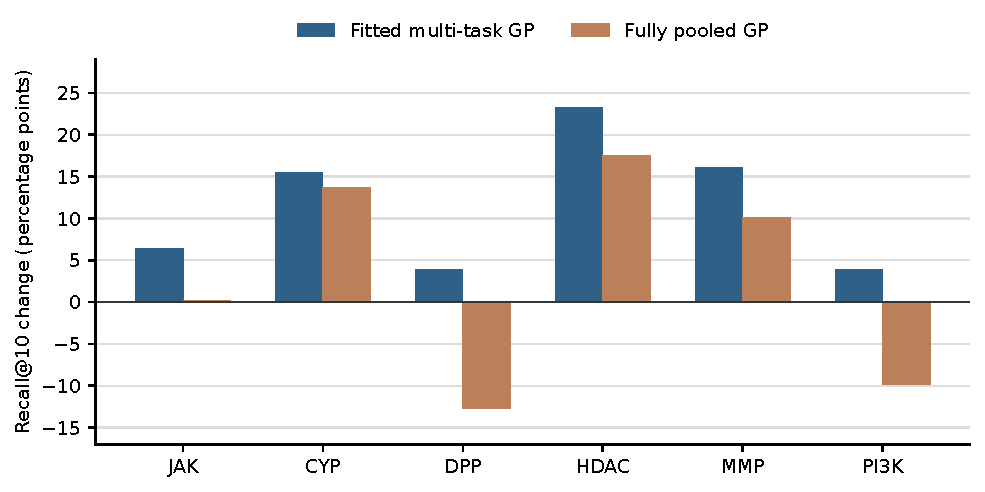
\includegraphics[width=0.8\linewidth]{generated/fig_uniform_family_recall.pdf}
\caption{Uniform-history Recall@10 gain against single-task BO for the six
BindingDB families (percentage points). Bars average the two budget-specific
contrasts for each family from the main text's budget-cell table. The figure
is descriptive; family-level inference is reported there.}
\label{fig:uniform-family}
\end{figure}

\paragraph{Coupling against family-level gain.} Comparing the median pairwise
correlation with each family's mean uniform-history gain, the pooled arm gives
Spearman \rhoPooledCoupling{} ($p=\,$\pPooledCoupling{}) and the fitted
multi-task arm \rhoMtCoupling{} ($p=\,$\pMtCoupling{}), over
$n=\nCouplingFamilies{}$ families. This is a post-hoc comparison on six points
and the two statistics are not independent, so we do not treat it as a test.
It is reported because it is the mechanism the pooling result implies: the arm
that assumes one shared activity function is the arm whose performance follows
how nearly that assumption holds, while estimating the coupling damps the
dependence.

\subsection{Datasets and preprocessing}
\label{app:data}

\begin{table}[htbp]
\centering\small
\begin{tabular}{lrrl}
\toprule
Dataset & Compounds & Targets & Response \\
\midrule
DOCKSTRING~\cite{dockstring2022} & 260{,}148 & 58 & Vina docking score \\
ChEMBL~\cite{chembl2019} & 3{,}970 & 4 & pIC$_{50}$ \\
BindingDB JAK~\cite{bindingdb2016} & $1{,}563\to904$ & 4 & pIC$_{50}$ \\
BindingDB CYP & $1{,}472\to335$ & 4 & pIC$_{50}$ \\
KIBA~\cite{tang2014kiba} & 904 / 899 / 843 & 4 each & KIBA score \\
\bottomrule
\end{tabular}
\caption{Dataset sizes and response scales. BindingDB counts are before and
after censoring filters; the KIBA entries are three pinned blocks.}
\label{tab:data}
\end{table}

BindingDB and ChEMBL IC$_{50}$ values in nanomolar units are converted to
pIC$_{50}$; KIBA scores retain their native scale. The selected shared
BindingDB blocks contain 904 JAK and 335 CYP compounds after filtering. To
avoid interpreting reporting ceilings as exact potencies, we exclude
compounds touching values present in more than $2\%$ of a BindingDB column;
this filter is disabled for KIBA. In DOCKSTRING, we use QED as an admission
criterion ($\mathrm{QED}\ge0.5$) rather than interpreting recovery of a
composite objective's known QED contribution as assay-driven discovery.
Stored data records include the source, transformation, censoring decision,
and block provenance.

\subsection{Campaign settings and statistical tests}
\label{app:statistics}

\begin{table}[htbp]
\centering\small
\begin{tabular}{lll}
\toprule
Setting & Value & Scope \\
\midrule
Fingerprint and kernel & ECFP4, 2048 bits; Tanimoto & All GP comparisons \\
Initial design & 10 compounds & Main campaigns \\
Batch size & 10 & Main campaigns \\
History per auxiliary target & 50 & Standard historical draws \\
Main history design & Uniform & Family comparison \\
Sensitivity history design & Top-10 withheld & Transfer diagnostics \\
Transfer budgets & 55--300 assay cells & Two per family \\
Initial-design budget & 60 assay cells & Secondary study \\
Historical-use options & 95 assay cells & Secondary study \\
Acquisition & Expected improvement & Except explicit controls \\
Seeds, principal controls & 32 per held-out target & $4\times32=128$ campaigns \\
Seeds, degradation ladder & 8 per held-out target & $4\times8=32$ campaigns \\
\bottomrule
\end{tabular}
\caption{Core campaign settings. Some diagnostic experiments vary history
coverage, budget, or acquisition as stated alongside their results. The two
seed counts correspond to two distinct stored run classes and are reported
separately throughout; see Section~\ref{app:degradation}.}
\label{tab:params}
\end{table}

Paired configurations use matching historical draws and initial compounds
where applicable; budgets and pairing invariants are audited. Paired
contrasts within a block use paired $t$-tests, while independent
configurations use Welch tests. Cross-family analyses average two budgets
within each family and apply a two-sided Wilcoxon signed-rank test across six
family effects. With six consistently signed nonzero effects, the minimum
exact two-sided $p$-value is $0.03125$. We report uncertainties and counts of
positive families alongside tests; exploratory tests were not adjusted for
family-wise multiplicity.

\section{Further transfer diagnostics}
\label{app:transfer-diagnostics}

\subsection{The C4 history-design comparison, per budget cell}
\label{app:design-cells}

Table~\ref{tab:design-cells} repeats the twelve budget cells in main-text
Table~3, without the family-level summary rows. Both budgets of a family draw the same historical
sample (Section~\ref{app:repro}), so these cells are not independent
replicates and no cross-family statistic is computed from them.

\begin{table}[htbp]
\caption{C4: Change in top-10 recall relative to \stl{} (percentage points)
for two assay budgets per family under withheld and uniform histories.
Every value is verified against the stored campaigns by
\texttt{scripts/family\_inference\_audit.py}.}
\label{tab:design-cells}
\centering\small
\begin{tabular}{llrrrr}
\toprule
 & & \multicolumn{2}{c}{\mt{} $-$ \stl{}} & \multicolumn{2}{c}{\pooled{} $-$ \stl{}} \\
\cmidrule(lr){3-4}\cmidrule(lr){5-6}
Cell & Coverage & withheld & uniform & withheld & uniform \\
\midrule
% summaries-exempt: per-cell grid; the CYP b111 and JAK b300 rows are the
% same runs the null-control table summarises, so the values coincide by
% construction. Generated per-cell output would duplicate tab:null.
CYP $b74$   & $45\%$ & $+8.44$  & $+19.77$ & $+14.22$ & $+17.42$ \\
CYP $b111$  & $45\%$ & $+9.69$  & $+11.25$ & $+17.50$ & $+10.00$ \\
DPP $b66$   & $50\%$ & $+6.02$  & $+4.69$  & $+1.95$  & $-11.17$ \\
DPP $b99$   & $50\%$ & $+2.66$  & $+3.05$  & $+2.11$  & $-14.30$ \\
HDAC $b83$  & $40\%$ & $+20.55$ & $+23.52$ & $+18.91$ & $+16.25$ \\
HDAC $b125$ & $40\%$ & $+21.72$ & $+22.89$ & $+25.39$ & $+18.67$ \\
JAK $b200$  & $17\%$ & $+5.78$  & $+4.45$  & $+2.97$  & $-0.31$ \\
JAK $b300$  & $17\%$ & $+7.66$  & $+8.28$  & $+5.70$  & $+0.78$ \\
MMP $b55$   & $60\%$ & $+12.34$ & $+17.03$ & $+16.33$ & $+10.47$ \\
MMP $b82$   & $60\%$ & $+16.09$ & $+15.16$ & $+18.75$ & $+9.69$ \\
PI3K $b130$ & $25\%$ & $-0.23$  & $+4.30$  & $-8.83$  & $-9.38$ \\
PI3K $b195$ & $25\%$ & $+1.72$  & $+3.52$  & $-8.36$  & $-10.23$ \\
% end-summaries-exempt
\bottomrule
\end{tabular}
\end{table}

\subsection{Legacy six-family null comparisons}
\label{app:permutation}

Table~\ref{tab:permutation} retains the earlier six-family permutation
results for sensitivity analysis. Legacy records do not document
whether permutation preceded history selection; these legacy results must
not be interpreted as preserving each observed history's response multiset.
The main text instead uses the verified historical-response permutation
and crossed-control runs described below. Each family contributes one number per column: the
mean over its two budget cells, which share a historical sample
(Section~\ref{app:repro}).

\begin{table}[htbp]
\centering\small
\begin{tabular}{lrrrrrr}
\toprule
 & \multicolumn{3}{c}{\mt{} $-$ \stl{}} & \multicolumn{3}{c}{\pooled{} $-$ \stl{}} \\
\cmidrule(lr){2-4}\cmidrule(lr){5-7}
Family & measured & permuted & difference & measured & permuted & difference \\
\midrule
CYP & $+15.51$ & $-2.46$ & $+17.97$ & $+13.71$ & $-15.74$ & $+29.45$ \\
DPP & $+3.87$ & $-2.58$ & $+6.45$ & $-12.73$ & $-23.09$ & $+10.35$ \\
HDAC & $+23.20$ & $-0.78$ & $+23.98$ & $+17.46$ & $-10.43$ & $+27.89$ \\
JAK & $+6.37$ & $+1.56$ & $+4.80$ & $+0.23$ & $-8.20$ & $+8.44$ \\
MMP & $+16.09$ & $-3.16$ & $+19.26$ & $+10.08$ & $-20.51$ & $+30.59$ \\
PI3K & $+3.91$ & $-0.82$ & $+4.73$ & $-9.80$ & $-19.22$ & $+9.41$ \\
\midrule
Mean & $+11.49$ & $-1.37$ & $+12.86$ & $+3.16$ & $-16.20$ & $+19.36$ \\
Families $>0$ & 6/6 & 1/6 & 6/6 & 4/6 & 0/6 & 6/6 \\
\bottomrule
\end{tabular}

\caption{Change in top-10 recall relative to \stl{} (percentage points) under
uniform histories in the legacy measured and permuted run classes.
Historical observation locations are matched. Preservation of the response
distribution within the observed historical sample was not independently
verified for this run class; it is not the new main-text null. Generated by
\texttt{scripts/family\_inference\_audit.py} from the stored campaigns.}
\label{tab:permutation}
\end{table}

The difference is positive in all six families for both arms
(\mt{}: \permMtGvalueShuf{} points, 95\% CI \permCiMtGvalueShuf{};
\pooled{}: \permPooledGvalueShuf{}, \permCiPooledGvalueShuf{}). Both reach
$p=\permPMtGvalueShuf{}$, which is the floor \permPFloor{} at $n=6$ rather
than a measure of how large the effect is; the paired $t$-values are
\permPtMtGvalueShuf{} and \permPtPooledGvalueShuf{}.

The recorded contrasts are retained as legacy diagnostics. Relative to the
Gaussian null, the measured-minus-permuted contrast differs by
\permMtNullDifference{} points for \mt{}
(95\% CI \permCiMtNullDifference{}).
For \pooled{}, the difference is \permPooledNullDifference{}
(95\% CI \permCiPooledNullDifference{}).
These estimates do not independently establish the absence of
observed-history distributional effects.

\paragraph{Covariance-free joint fitting (C2).}
Under randomized auxiliary responses and withheld histories, the JAK
\mtzero{} gain is \valMechJakMtRZero{} $\pm$ \semMechJakMtRZero{}
points, compared with \valMechJakMt{} $\pm$ \semMechJakMt{} for \mt{}.
On CYP, the corresponding gains are \valMechCypMtRZero{} $\pm$
\semMechCypMtRZero{} for \mtzero{} and \valMechCypPooled{} $\pm$
\semMechCypPooled{} for \pooled{}.
These are means $\pm$ SEM over \nMechJakMtRZero{} campaigns per
comparison; they reproduce the C2 values cited in the main text.

\subsection{Verified historical-response permutation and crossed fits}
\label{app:crossed}

The new null draws historical locations first, then permutes the fifty
observed responses within each auxiliary target, separately for each held-out
primary target and repeat. Permutations remain fixed through each campaign.
The four crossed conditions are defined in main-text C2; every locked fit
retains the donor's coupling, noise-to-signal ratio, signal variance, per-task
means and scales, inner GP normalization, and numerical jitter. Reconditioning
reuses the donor's Cholesky factor and changes only the response coefficients.
For fixed covariance $K_\theta$, noise $\Lambda_\theta$, and test covariance
$k_*$, the posterior variance
\[
v_*=k_{**}-k_*^\top(K_\theta+\Lambda_\theta)^{-1}k_*
\]
does not depend on conditioning responses. This is a standard GP property;
the contribution is its controlled use to distinguish routes of auxiliary
response information in molecular screening, not a new variance identity.

All six panels use the original two budgets, four primary targets, and
32 repeats per target. A larger-budget trajectory supplies the smaller-budget
prefix, reproducing the deterministic truncated-batch policy exactly.
The two-repeat smoke phase checks all panels and budgets without selecting
experiments by their effect sizes. Same-condition locked posteriors reproduce
their donors, and locked predictive variances are exactly unchanged under
response replacement. Independent reconstruction confirms zero discrepancy
from the stored single-task and measured-response recall vectors at both
budgets. The observed response multisets are identical; moment discrepancies
are at floating-point rounding level. Selected indices, permutation source
indices, input hashes, parameter snapshots, and replay records are saved in
\texttt{results/crossed\_auxiliary\_v1/}.

The primary sequential comparison is $MM-PP$: $\crossPrimary{}$ points,
95\% CI $\crossPrimaryCi{}$, positive in $\crossPrimaryPositive{}/6$
families, with two-sided Wilcoxon $p=\crossPrimaryP{}$.
Other conditional contrasts and their interaction are descriptive. Budgets,
primary targets, and repeated seeds do not create additional independent
family observations. Parameters supplied by the measured donor retain
response information even when conditioning responses are permuted.

Replays evaluate all policies at every batch boundary on shared \stl{}
and $MM$ trajectories, with common candidates, incumbents, and tie-breaking.
Future primary activities score the proposed batches retrospectively and
never enter the fitting function. Rounds are averaged within campaigns,
then budgets and campaigns within each family. These summaries describe
one-step selection on fixed histories, while sequential-policy contrasts
include feedback from differing acquired observations. They do not identify
unique causal mechanisms or assign causal fractions to final recall.

\begin{table}[htbp]
\centering\small
\begin{tabular}{lrrrr}
\toprule
Family & $\mathrm{MM}$ $-$ \stl{} & $\mathrm{MP}$ $-$ \stl{} & $\mathrm{PM}$ $-$ \stl{} & $\mathrm{PP}$ $-$ \stl{} \\
\midrule
JAK & $+6.37$ & $-2.07$ & $+4.49$ & $+1.99$ \\
CYP & $+15.51$ & $-13.09$ & $+9.18$ & $-2.38$ \\
DPP & $+3.87$ & $-1.76$ & $+0.70$ & $-1.21$ \\
HDAC & $+23.20$ & $-3.75$ & $+5.59$ & $-3.36$ \\
MMP & $+16.09$ & $-10.70$ & $+3.98$ & $-2.54$ \\
PI3K & $+3.91$ & $-3.52$ & $-1.33$ & $+0.43$ \\
\midrule
Mean & $+11.49$ & $-5.81$ & $+3.77$ & $-1.18$ \\
\bottomrule
\end{tabular}

\caption{Verified crossed-control recall gains over single-task BO, in
percentage points. Each family averages its two budgets; condition notation
matches main-text Table~1. The complete per-budget outcomes and additional
replay metrics are in the independent summary JSON.}
\label{tab:crossed-supp}
\end{table}

\subsection{Uncertainty trajectory behind the C3 scale}

Joint fitting reduces mean posterior standard deviation from $0.643$ to
$0.558$ on JAK and from $0.629$ to $0.522$ on CYP when $r=0$. On JAK, the
early fitted-multi-task/single-task uncertainty ratio is $0.80$ at 50 primary
observations and rises later in the campaign. The fixed EI scale used in the
main text is thus motivated by an early diagnostic; it is not intended to
match the complete uncertainty trajectory, and it was not selected by
maximizing recall. The corresponding CYP sweep over $c\in[0.35,20]$ is
reported in the main text as an upper bound. This comparison does not
establish improved uncertainty calibration. Existing held-out residual
probes give standardized-residual standard deviations above one on both
JAK and CYP, rather than the approximately 0.80 value expected from a
calibration explanation of JAK's compression. Changed JAK selections also
show no clear separation in chemical isolation. These are supporting
diagnostics, not causal identifications (\texttt{results/mechanism\_probes.json}).
The JAK scale $c=0.80$
yields a recall gain of \valScaleMatchedJak{} $\pm$
\semScaleMatchedJak{} points over \nScaleMatchedJak{} campaigns.

\subsection{High-coverage CYP history-design ladder}

The twelve budget cells behind control C4, and the family-level aggregates
computed from them, are given in the main text; this section records the
separate high-coverage CYP diagnostic that motivates them.

That diagnostic uses \emph{randomized} auxiliary responses on a block whose
auxiliary history covers an unusually large share of the campaign library, so
the pooled model's treatment of already-measured compounds is maximally
visible. Pooled gains at 30, 75, 150 and 300 randomized historical rows are
$-1.25$, $+2.34$, $+10.55$ and $+22.97$ points under withholding: a
monotone ``more history helps more'' curve produced from data containing no
transferable information whatsoever. Holding the model, the budget, the seed
set and the number of historical rows fixed, and changing only the selection
rule from withheld to uniform, reverses the 300-row result to $-23.05$
points. A permutation null under uniform history, which preserves the
auxiliary marginal distributions and breaks only the compound alignment,
gives $-19.69$ points. The $46$-point swing is attributable to the selection
rule alone.

These are randomized-response diagnostics on one high-coverage block. They
are not comparable to the fitted-model, measured-response comparison across
the six families in the main text, and we do not pool them with it.

\paragraph{Calibration of the auxiliary-response-free avoidance control.}
The single-task policy multiplies EI at historical compounds by $W$, leaving
EI elsewhere unchanged. The penalty is calibrated to the pooled model's
campaign-wide history-selection ratio, without using auxiliary responses
or optimizing recall. Calibrated runs are separate from the high-coverage
ladder above and should not be treated as the same campaigns.
At coverage \avoidCoverageHundred{}, $W=$\avoidWHundred{} gives a
selection ratio of \avoidAchievedRatioHundred{} against the target
\avoidTargetRatioHundred{}. Its withheld-to-uniform recall change is
\avoidRecallSwingHundred{} points, compared with
\pooledRecallSwingHundred{} for full pooling, reproducing
\avoidRecallFracHundred{} of the change. Its recall-curve AUC change is
\avoidAucSwingHundred{}, or \avoidAucFracHundred{} of the pooled AUC change.
At coverage \avoidCoverageFifty{}, $W=$\avoidWFifty{} gives a ratio of
\avoidAchievedRatioFifty{} against \avoidTargetRatioFifty{}; the recall
change is \avoidRecallSwingFifty{} points, reproducing
\avoidRecallFracFifty{} of \pooledRecallSwingFifty{}. The AUC change is
\avoidAucSwingFifty{}, or \avoidAucFracFifty{} of the pooled AUC change.
Each condition uses \avoidCampaignsHundred{} campaigns. These ratios
summarize behavioral reproduction, not a causal partition of the pooled effect.

\section{Assay allocation and library overlap}
\label{app:sharing}

Complementary experiments on KIBA~\cite{tang2014kiba},
ChEMBL~\cite{chembl2019}, and DOCKSTRING~\cite{dockstring2022}
examine assay allocation, historical-data reuse,
and initial compound selection. KIBA scores
are retained on their original scale, while
DOCKSTRING provides simulated docking scores
rather than experimental activities.
These analyses distinguish experimental activities, KIBA scores on their
original scale, and simulated DOCKSTRING docking scores.

Existing historical measurements do not consume new
primary-target assays. By contrast, allocating new assays
to related targets reduces primary-target predictive rank
correlation in the tested settings. Reusing history is most
useful when primary data are scarce and offers little benefit
on low-overlap ChEMBL; history can also guide initial
compound selection without entering the GP. These supplementary
analyses use predictive rank correlation or recall-curve AUC,
not the main Recall@10 metric (Sections~S3--S4).


Allocating \emph{new} assays and reusing \emph{existing} history are
different interventions with different cost models, and Table~\ref{tab:sharing}
reports them separately. Both panels use the same endpoint: Spearman rank
correlation between predicted and measured primary-target activity on the
held-out compounds of the primary target. That is a \emph{predictive-ranking}
quantity, not the Recall@10 endpoint of the BO campaigns.

\begin{table}[htbp]
\centering\small
\textbf{(a) Allocating a fixed budget of new assays}\\[3pt]
\begin{tabular}{llcr}
\toprule
Dataset & Design & $n$ & $\Delta\rho$ vs.\ \stl{} \\
\midrule
DOCKSTRING (21 kinases) & Spread  & 80 & $-0.056$ \\
DOCKSTRING (21 kinases) & Blocked & 80 & $-0.191$ \\ % was -0.189; transfer/summary/80/headroom = -0.1907
JAK block & Spread & 80 & $-0.127\pm0.014$ \\ % TODO UNSOURCED: no h1_split artefact for JAK; only -0.127 in tree is DOCKSTRING ABL1 n=80 BLOCKED. Rerun or drop this row.
CYP block & Spread & 80 & $-0.045\pm0.008$ \\ % dense_block_h1_cyp.json h1_split/80
\bottomrule
\end{tabular}

\medskip
\textbf{(b) Reusing $H=50$ existing measurements per auxiliary target}\\[3pt]
\begin{tabular}{lrrrr}
\toprule
& \multicolumn{4}{c}{$\Delta\rho$ at primary training size $n$}\\
\cmidrule(lr){2-5}
Dataset & $n=10$ & $n=20$ & $n=40$ & $n=80$ \\
\midrule
DOCKSTRING (4 kinases)      & $+0.310$ & $+0.233$ & ---      & $+0.086$ \\
ChEMBL (separate libraries) & $+0.001$ & $-0.020$ & ---      & $-0.007$ \\
BindingDB JAK block         & $+0.101$ & $+0.086$ & $+0.049$ & ---      \\
BindingDB CYP block         & $+0.256$ & $+0.181$ & $+0.117$ & ---      \\
\bottomrule
\end{tabular}
\caption{Two resource-use comparisons, both measured as a change in
primary-target held-out Spearman rank correlation $\Delta\rho$.
\textbf{(a)} The cost of \emph{buying} assays on relatives: a fixed new-assay
budget is spent on the primary target alone (\stl{}) or divided across the
block, either evenly (\emph{spread}) or concentrated on one relative
(\emph{blocked}). Every tested panel loses ranking accuracy, so the extra
auxiliary assays do not repay the primary-target observations they displace.
\textbf{(b)} The value of \emph{free} history: each auxiliary target
contributes $H=50$ already-collected measurements at no budget cost, and the
entry is the multi-task GP's $\Delta\rho$ over a single-task GP trained on
the same $n$ primary observations. The two dataset groups were run on
different grids ($n\in\{10,20,80\}$ for DOCKSTRING and ChEMBL,
$n\in\{10,20,40\}$ for the BindingDB blocks), so a dash marks a grid point
that was never run, not a failed or omitted result. Reuse is worth most when
the primary target is coldest, decays as primary data accumulates, and is
near zero on ChEMBL, where the four libraries share almost no compounds
(pairwise overlap $\le1.7\%$).}
\label{tab:sharing}
\end{table}

History reuse is stronger in shared-compound panels. Complementary chemical
coverage alone does not account for the weaker separate-library ChEMBL
result: the mean ratio of auxiliary to own nearest-neighbour similarity there
is $0.53$, so the auxiliary libraries do occupy adjacent chemistry, yet the
borrowed rows still buy almost nothing.

\section{Secondary study: initial-design use of history}
\label{app:secondary}

Related-target measurements can select the first compounds without entering
the GP posterior. The \auxtop{} rule selects high-activity auxiliary
compounds after standardization; \auxnn{} also includes nearby chemical
analogues; \maxmin{} selects diverse compounds without assay responses.
These experiments address the practical use of existing data, not an
additional control for transfer attribution.

\subsection{Held-out choice between seeding and transfer}
\label{sec:res-rule}

We compare \emph{abstain} (random initial design, single-task BO),
\emph{seed} (initialize from high-scoring history), and \emph{transfer}
(multi-task GP). A simple linear rule selects among them using estimated
target correlation. Each of 18 KIBA blocks is held out in turn while the rule
is fitted to the other 17. The history protocol is evaluated both ways
because uniform and withheld sampling can favour different choices.

\begin{table}[htbp]
\centering\small
\begin{tabular}{llrrrr}
\toprule
History & Policy & Mean $\Delta$AUC & Positive & vs.\ best fixed & $p$ \\
\midrule
Uniform  & always abstain   & $+0.0000$ & $0/18$  &           &        \\
         & always transfer  & $+0.1089$ & $12/18$ &           &        \\
         & \textbf{always seed} & $\mathbf{+0.1293}$ & $\mathbf{17/18}$ & --- & \\
         & rule (held out)  & $+0.1245$ &         & $-0.0048 \pm 0.0027$ & $0.25$ \\
         & best per block (hindsight) & $+0.1421$ &        &           & \\
\midrule
Withheld & always abstain   & $+0.0000$ & $0/18$  &           &        \\
         & always seed      & $+0.0350$ & $10/18$ &           &        \\
         & \textbf{always transfer} & $\mathbf{+0.0494}$ & $\mathbf{12/18}$ & --- & \\
         & rule (held out)  & $+0.0549$ &         & $+0.0055 \pm 0.0040$ & $0.22$ \\
         & best per block (hindsight) & $+0.0660$ &        &           & \\
\bottomrule
\end{tabular}
\caption{Leave-one-block-out comparison over 18 KIBA blocks. The rule is
compared with the best fixed policy; only three uniform-history and six
withheld-history blocks differ from that fixed choice. The hindsight row
selects on noisy observed outcomes and is biased upward; it is not an
achievable bound for a learned rule.}
\label{tab:rule}
\end{table}

Under uniform history the fixed seeding strategy gains $+0.1293$ recall AUC
relative to random initialization and is positive on 17 of 18 blocks; under
withholding, fitted-model transfer is the better fixed strategy. Note that
this reverses the ordering of \emph{seed} and \emph{transfer}, so the
history-design sensitivity of control C4 is not confined to the pooled GP: it
also changes which practical recipe a benchmark would recommend. The
correlation-based chooser does not clearly improve on the best fixed policy
($-0.0048\pm0.0027$ uniform, $p=0.25$; $+0.0055\pm0.0040$ withheld,
$p=0.22$), and these comparisons rest on only three and six discordant
blocks respectively.

\subsection{Dependence on historical sample size}
\label{sec:res-panel}

\begin{table}[htbp]
\centering\small
\begin{tabular}{lrrlrlrc}
\toprule
Panel & $H$ & blocks & $\rho$ range & crossing & 95\% CI & mean gain & $>0$ \\
\midrule
KIBA      & 50 & 18 & $-0.01$ to $+0.43$ & $+0.081$ & $[0.01, 0.13]$ & $+0.062$ & $12/18$ \\
KIBA      & 20 & 18 & $-0.01$ to $+0.43$ & $+0.262$ & $[0.17, 0.48]$ & $-0.018$ & $7/18$ \\
BindingDB & 50 & 6  & $+0.26$ to $+0.65$ & $+0.155$ & $[0.06, 0.35]$ & $+0.110$ & $6/6$ \\
BindingDB & 20 & 6  & $+0.26$ to $+0.65$ & $+0.421$ & $[0.35, 0.51]$ & $+0.033$ & $4/6$ \\
\bottomrule
\end{tabular}
\caption{Seeding-threshold estimates for different historical sample sizes
$H$, with mean recall-AUC gain relative to random initialization. Crossings
are defined on the effective target-coupling axis.}
\label{tab:panel}
\end{table}

The signal needed for history-based seeding depends on how many
related-target measurements are available. On KIBA the estimated crossing
rises from about $0.08$ to $0.26$ as history falls from 50 to 20
measurements, and the BindingDB estimates move in the same direction. These
exploratory thresholds are conditional on the history size and the evaluated
panels; they are not universal target-similarity rules.

The expanded initial-design sweeps, degradation ladders, weakly coupled
target scans, and within-block threshold fits are retained in the extended
analysis records released with the code.

\section{Additional acquisition diagnostic}
\label{app:acquisition}

Greedy selection uses the predicted activity without the uncertainty term in
EI. Its comparisons with randomized and measured auxiliary responses are
mixed, so these experiments do not support an explanation resting on
uncertainty alone.

\begin{table}[htbp]
\centering\small
\begin{tabular}{llrrr}
\toprule
Block & Acquisition & $q$ & \mt{} $-$ \stl{} & \pooled{} $-$ \stl{} \\
\midrule
JAK & EI     & 0 & $+2.8$ ($p=0.037$) & $+1.9$ (n.s.) \\
JAK & EI     & 1 & $+7.2$ ($p<0.001$) & $+6.2$ ($p<0.001$) \\
JAK & greedy & 0 & $+3.1$ (\textbf{n.s.}) & $+7.5$ (n.s.) \\
JAK & greedy & 1 & $\mathbf{+16.2}$ ($p=0.008$) & $+4.7$ (n.s.) \\
\midrule
CYP & EI     & 0 & $+1.6$ (n.s.) & $\mathbf{+14.7}$ ($p<0.001$) \\
CYP & EI     & 1 & $+11.9$ ($p<0.001$) & $+20.9$ ($p<0.001$) \\
CYP & greedy & 0 & $-2.5$ (n.s.) & $\mathbf{-20.6}$ ($p=0.001$) \\
CYP & greedy & 1 & $+4.4$ (n.s.) & $\mathbf{-7.5}$ ($p=0.081$) \\
\bottomrule
\end{tabular}
\caption{The same comparisons under expected improvement, which uses
predicted activity and uncertainty, and greedy selection, which uses
predicted activity alone. With randomized auxiliary values, EI shows a clear
positive gain on CYP for the pooled model while the mean-only results are
mixed, consistent with the history-avoidance account, since avoidance acts
through the variance term that greedy selection discards.}
\label{tab:greedy}
\end{table}

\section{Reproducibility and provenance}
\label{app:repro}

The evidence package includes stored campaign outcomes, input blocks,
analysis scripts, provenance fields, and a SHA-256 manifest. Reported tables
and figures are regenerated from stored outcomes; full campaign reruns
require the original affinity dumps. The audits check seed inventories,
budget and pairing invariants, preprocessing transformations, and agreement
of generated statistics. All 26 audited campaign re-runs reproduced their
stored summaries to $10^{-9}$, and all 20 checked preprocessing quantities
matched their source blocks. The package records statistical test settings
and exactness, so results are not reconstructed by copying rounded values
from the manuscript.

\paragraph{Exact pairing of the null comparisons.}
Each run stores SHA-256 digests of three streams in cell order: the drawn
historical indices, the initial design, and the auxiliary values handed to the
arms. A control is paired with its reference only if the first two digests
match and the third differs, which is a stronger check than the equal history
size and coverage statistics it replaces --- two different draws of the same
size reach the same coverage routinely. Re-running all 36 cells of the
six-family comparison (12 cells $\times$ measured, permuted, Gaussian) gives
identical history and initial-design digests across the three conditions in
every cell, and pairwise distinct auxiliary-value digests in every cell.

Grouping the twelve budget cells by history digest yields exactly six groups,
one per family: the two budgets of a family were measured on the same
historical compounds from the same initial designs, because the history draw
is a function of the seed, the held-out target, the repeat and the library,
and not of the budget. This is the basis for treating the six families, rather
than the twelve budget cells, as the units of cross-family inference.

\section{Panel selection and data exclusions}
\label{app:panel-screen}

For the secondary weak-correlation screen, four-target combinations were
sampled from 173 KIBA targets with at least 160 measurements. Eligible blocks
had at least 300 shared compounds and were selected across six correlation
ranges while limiting target overlap. The resulting 18 blocks contained
428--433 compounds, with target correlations from $-0.015$ to $+0.433$.
Because blocks were stratified by correlation, they are not representative of
the full KIBA panel. Davis was excluded because 68 compounds cannot support
the required 150 distinct historical compounds; an independently identified
potency-direction error did not affect any reported result.

\bibliographystyle{plain}
\bibliography{mybibliography}
\end{document}
